%%%%%%%%%%%%%%%%%%%%%%%%%%%%%%%%%%%%%%%%%%%%%%%%%%%%%%%%%%%%%%%%%%%%%%%%%%%%%%%%
%%%%%%%%%%%%%%%%%%   Vorlage für eine Abschlussarbeit   %%%%%%%%%%%%%%%%%%%%%%%%
%%%%%%%%%%%%%%%%%%%%%%%%%%%%%%%%%%%%%%%%%%%%%%%%%%%%%%%%%%%%%%%%%%%%%%%%%%%%%%%%

% Erstellt von Maximilian Nöthe, <maximilian.noethe@tu-dortmund.de>
% ausgelegt für lualatex und Biblatex mit biber

% Kompilieren mit
% latexmk --lualatex --output-directory=build thesis.tex
% oder einfach mit:
% make

\documentclass[
  tucolor,       % remove for less green,
  BCOR=12mm,     % 12mm binding corrections, adjust to fit your binding
  parskip=half,  % new paragraphs start with half line vertical space
  open=any,      % chapters start on both odd and even pages
  cleardoublepage=plain,  % no header/footer on blank pages
]{tudothesis}


% Warning, if another latex run is needed
\usepackage[aux]{rerunfilecheck}

% just list chapters and sections in the toc, not subsections or smaller
\setcounter{tocdepth}{1}

%------------------------------------------------------------------------------
%------------------------------ Fonts, Unicode, Language ----------------------
%------------------------------------------------------------------------------
\usepackage{fontspec}
\defaultfontfeatures{Ligatures=TeX}  % -- becomes en-dash etc.

% load english (for abstract) and ngerman language
% the main language has to come last
\usepackage[american, ngerman]{babel}

% intelligent quotation marks, language and nesting sensitive
\usepackage[autostyle]{csquotes}

% microtypographical features, makes the text look nicer on the small scale
\usepackage{microtype}

%------------------------------------------------------------------------------
%------------------------ Math Packages and settings --------------------------
%------------------------------------------------------------------------------

\usepackage{amsmath}
\usepackage{amssymb}
\usepackage{mathtools}

% Enable Unicode-Math and follow the ISO-Standards for typesetting math
\usepackage[
  math-style=ISO,
  bold-style=ISO,
  sans-style=italic,
  nabla=upright,
  partial=upright,
]{unicode-math}
\setmathfont{Latin Modern Math}

% nice, small fracs for the text with \sfrac{}{}
\usepackage{xfrac}


%------------------------------------------------------------------------------
%---------------------------- Numbers and Units -------------------------------
%------------------------------------------------------------------------------

\usepackage[
  locale=DE,
  separate-uncertainty=true,
  per-mode=symbol-or-fraction,
]{siunitx}
\sisetup{math-micro=\text{µ},text-micro=µ}

%------------------------------------------------------------------------------
%-------------------------------- tables  -------------------------------------
%------------------------------------------------------------------------------

\usepackage{booktabs}       % \toprule, \midrule, \bottomrule, etc

%------------------------------------------------------------------------------
%-------------------------------- graphics -------------------------------------
%------------------------------------------------------------------------------

\usepackage{graphicx}
% currently broken
% \usepackage{grffile}

% allow figures to be placed in the running text by default:
\usepackage{scrhack}
\usepackage{float}
\floatplacement{figure}{htbp}
\floatplacement{table}{htbp}

% keep figures and tables in the section
\usepackage[section, below]{placeins}


%------------------------------------------------------------------------------
%---------------------- customize list environments ---------------------------
%------------------------------------------------------------------------------

\usepackage{enumitem}

%------------------------------------------------------------------------------
%------------------------------ Bibliographie ---------------------------------
%------------------------------------------------------------------------------

\usepackage[
  backend=biber,   % use modern biber backend
  autolang=hyphen, % load hyphenation rules for if language of bibentry is not
                   % german, has to be loaded with \setotherlanguages
                   % in the references.bib use langid={en} for english sources
]{biblatex}
\addbibresource{references.bib}  % the bib file to use
\DefineBibliographyStrings{german}{andothers = {{et\,al\adddot}}}  % replace u.a. with et al.


% Last packages, do not change order or insert new packages after these ones
\usepackage[pdfusetitle, unicode, linkbordercolor=tugreen, citebordercolor=tugreen]{hyperref}
\usepackage{bookmark}
\usepackage[shortcuts]{extdash}

%------------------------------------------------------------------------------
%-------------------------    Angaben zur Arbeit   ----------------------------
%------------------------------------------------------------------------------

\author{Yanick Sebastian Kind}
\title{Mn-Verunreinigungen in Graphen: Eine Tight Binding Modellierung}
\date{2022}
\birthplace{Fairfield}
\chair{Lehrstuhl für Theoretische Physik 2}
\division{Fakultät Physik}
\thesisclass{Bachelor of Science}
\submissiondate{XX. Juli 2022}
\firstcorrector{Prof.~Dr.~Anders}
\secondcorrector{Prof.~Dr.~Uhrig}

% tu logo on top of the titlepage
\titlehead{
\includegraphics[height=1.5cm]{logos/tu-logo.pdf}}

\newcommand{\compconj}[1]{%
  \overline{#1}%
}

\begin{document}
\frontmatter
\thispagestyle{empty}
\setcounter{page}{2}
\section*{Hinweise}
Empfohlen wird die Verwendung dieser Vorlage mit der jeweils aktuellsten TeXLive Version (Linux, Windows) bzw. MacTeX Version (MacOS).
Aktuell ist dies TeXLive 2021. Download hier:
\begin{center}
  \ttfamily\url{https://www.tug.org/texlive/}
\end{center}

Die Vorlage \texttt{thesis.tex} ist für die Kompilierung mit \texttt{lualatex} ausgelegt, mit wenigen Anpassungen kann sie aber auch mit \texttt{pdflatex} oder \texttt{xelatex} verwendet werden.
Die Dokumentenklasse \texttt{tudothesis.cls} kann mit allen drei Programmen verwednet werden.

Achten Sie auch auf die Kodierung der Quelldateien.
Bei Verwendung von Xe\LaTeX\ oder Lua\LaTeX\ (empfohlen) müssen die
Quelldateien UTF-8 kodiert sein.
Bei Verwendung von pdf\LaTeX\ nutzen Sie die Pakete \texttt{inputenc} und \texttt{fontenc} mit der korrekten Wahl der Kodierungen.

Eine aktuelle Version dieser Vorlage steht unter 
\begin{center}
  \ttfamily\url{https://github.com/maxnoe/tudothesis}
\end{center}
zur Verfügung.

Alle verwendeten Pakete werden im \LaTeX{} Kurs von Pep et al.\ erklärt:
\begin{center}
  \ttfamily\url{http://toolbox.pep-dortmund.org/notes}
\end{center}

Für Rückmeldungen und bei Problemen mit der Klasse oder Vorlage, bitte ein \emph{Issue} auf GitHub aufmachen oder eine Email an
\href{mailto:maximilian.noethe@tu-dortmund.de}{maximilian.noethe@tu-dortmund.de} schreiben.

Wenn Sie die Dokumentenklasse mit der Option \texttt{tucolor} laden, werden verschiedene Elemente in TU-Grün gesetzt.

\maketitle

% Gutachterseite
\makecorrectorpage

% hier beginnt der Vorspann, nummeriert in römischen Zahlen
\thispagestyle{plain}

\section*{Kurzfassung}
In dieser Arbeit wird eine einzelne Mangan-Verunreinigung in Graphen mittels eines Tight Binding Modells in einer nächsten-Nachbarn Näherung
ohne die Coulomb-Wechselwirkung zwischen den Elektronen betrachtet.
Ein besonderes Augenmerk liegt dabei auf den Kopplungen zwischen den fünf $3d$-Orbitalen des Mangans und den $p_z$-Orbitalen der drei umliegenden 
Kohlenstoffatome, welche mittels Slater-Koster-Integralen beschrieben wird.
Das Ziel dieser Arbeit ist die Berechnung der Hybridisierungsfunktion der $3d$-Orbitale des Mangans und die Untersuchung 
des Einflusses der Graphenbänder auf die $3d$ Elektronen des Mangans, da es in dem Experiment, beschrieben in \cite{doi:10.1021/acsnano.1c00139}, Hinweise auf einen Kondo-Effekt gibt. 
Einerseits wird diese mittels Bewegungsleichungen für Greensche Funktionen ermittelt.
Anderseits wird die Symmetrie des Problems mittels gruppentheoretischen Überlegungen ausgenutzt, um die Hybridisierungsfunktion zu bestimmen.
Dabei wird gezeigt, welche $3d$-Orbitale mischen und im Zuge dessen ein effektives Drei-Bänder Modell nachgewiesen.
\section*{Abstract}
\begin{foreignlanguage}{english}
In the present work a single Mangan impurity in Graphene will be discussed with a nearest neighbour Tight Binding model, where
the Coulomb Interaction will be neglected.
Particular attention is paid to the coupling between the five $3d$-orbitals of the Manganese and the $p_z$-orbitals of the three
sourrounding Carbon atoms, which will be described by Slater-Koster integrals.
The aim of this thesis is the calculation of the hybridisation function of the $3d$-orbitals of the Manganese.
One method is to use equations of motion for Green's functions. 
The hybridisation function is also determined by involving group theory to use the symmetrie of the problem.
In the process the mixing of the $3d$-orbitals and a three band model will be verified. 
\end{foreignlanguage}
\tableofcontents

\mainmatter
% Hier beginnt der Inhalt mit Seite 1 in arabischen Ziffern
\chapter{Einleitung}
\section{Motivation}
\label{sec:motivation}
Motiviert wurde diese Arbeit durch den Artikel \cite{doi:10.1021/acsnano.1c00139}, aus welchem jegliche Informationen dieses 
Abschnitts entnommen wurden.
In dem dort behandelten Experiment wird mittels ultra-niederenergetischer Ionenimplantation
(\textit{ultralow-energy ion implantation}) Mangan (Mn) in eine einzelne Graphenstörstelle, wobei sich das Graphen auf einem Kupfersubstrat befindet, eingesetzt.
Es wurden die Positionen des Mn im Bezug auf die Moiré-Superstruktur (Abbildung \ref{fig:ascnano_structure}), die elektronischen und magnetischen Eigenschaften und die Konzentration der Mn-Defekte
untersucht.
Die Moiré-Superstruktur bildet sich aus, da die vertikale Ausrichtung zwischen dem Graphen und dem Kupfer kontinuierlich variiert.
\begin{figure}[H]
    \centering
    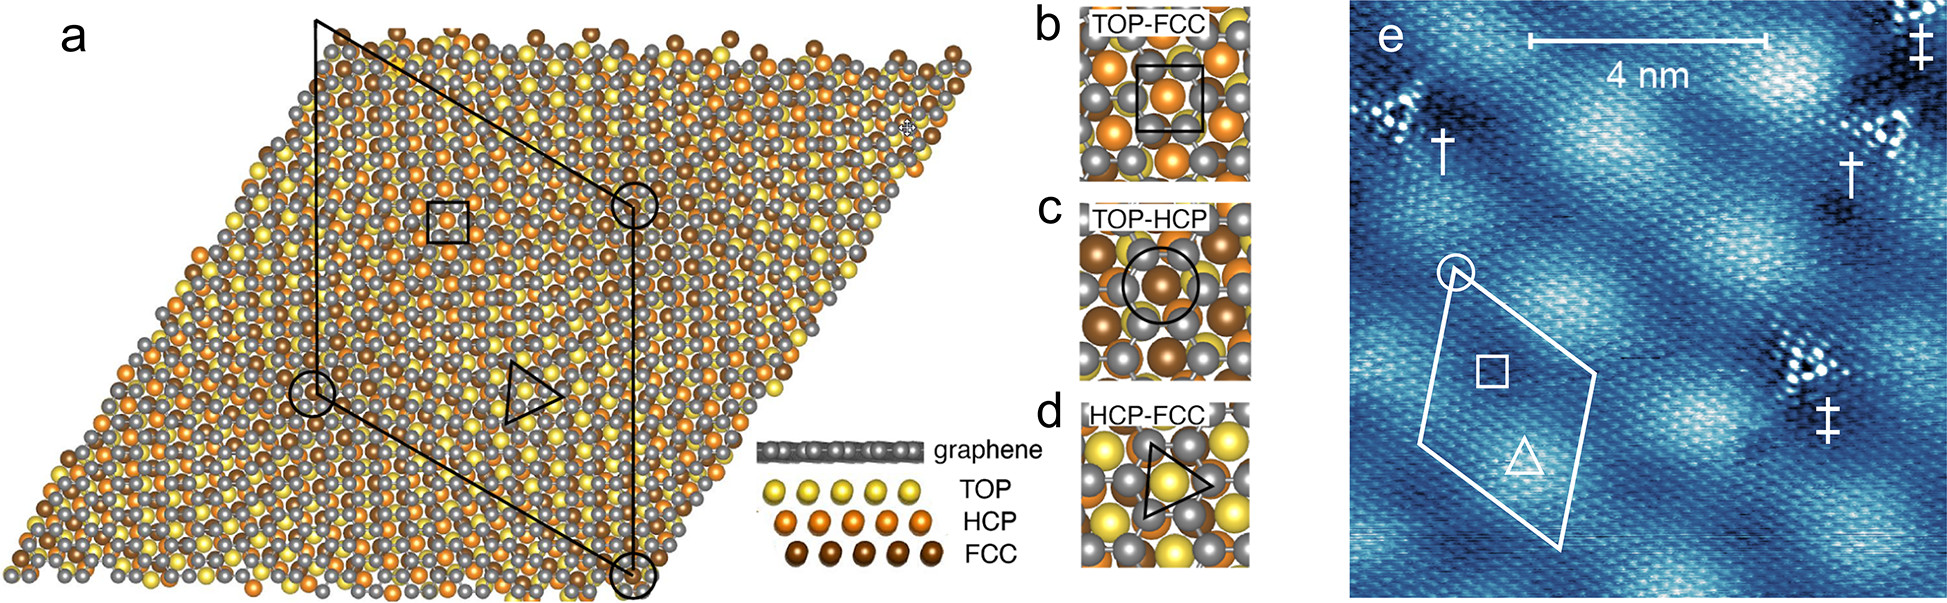
\includegraphics[width = \textwidth]{Plots/images_large_nn1c00139_0002.jpeg}
    \caption{(a) zeigt die Moiré-Superstruktur. Durch kontinuierliche Variation der der Ausrichtung 
    zwischen dem Kupfer und Graphen, entstehen Hochsymmetriepunkte bezüglich des Stapelns (b-d).
    Diese Hochsymmetriepunkte und somit auch die Moiré-Superstruktur können mittels Rastertunnelmikroskopie (RTM) 
    visualisiert werden, womit eine zweidimensionale Periodizität ersichtlich wird (e).
    (Abbildung entnommen  aus \cite{doi:10.1021/acsnano.1c00139})}
    \label{fig:ascnano_structure}
\end{figure}
Graphen mit Mn-Störstellen eignet sich für die Untersuchung elektrischer und magnetischer Eigenschaften, da die Bänder bei einer Konzentration von ca. $\qty{0.04}{\percent}$ 
die Dirac-Eigenschaften beibehalten und es somit ein ideales System für das Studieren der Interaktion
zwischen lokalen magnetischen Momenten und den Dirac-Elektronen (siehe Abschnitt \ref{sec:propertiesofgraphene}) darstellt.
Abbildung \ref{fig:ascnano_structure}a zeigt die Probe auf atomarer Ebene, worin auch die Moiré-Superstruktur deutlich wird.
Die Stellen mit hoher Symmetrie bezüglich des Stapelns des Graphens auf dem Substrat werden in 
Abbildung \ref{fig:ascnano_structure}b-d aufgezeigt.
Diese bilden wiederum ein zweidimensionales Gitter (Abb. \ref{fig:ascnano_structure}e).
Aufgrund der kurzen Reichweite der Bindungen, welche Graphen charakterisiert, und des großen Radius von Mn im Vergleich zur 
Kohlenstoff-Fehlstelle (C-Fehlstelle) entweicht das Mn senkrecht zur Graphenebene.
Es kann sich zwischen das Graphen und das Substrat oder zwischen Graphen und Vakuum (nach außen gerichtet) entweichen. 
Jedoch wurden mögliche nach außen gerichtete Anordnung nur mit einer Wahrscheinlichkeit, 
welche um mehr als zwei Größenordnungen kleiner ist, beobachtet.
Dies liegt daran, dass die Konfiguration mit dem nach außen gerichteten Mn eine höhere Energie aufweist und somit instabiler ist.
Während das Mn zum Kupfersubstrat entweicht, nehmen die C um diese Störstelle herum eine nach außen gerichtete Positon ein.
\begin{figure}
    \centering
    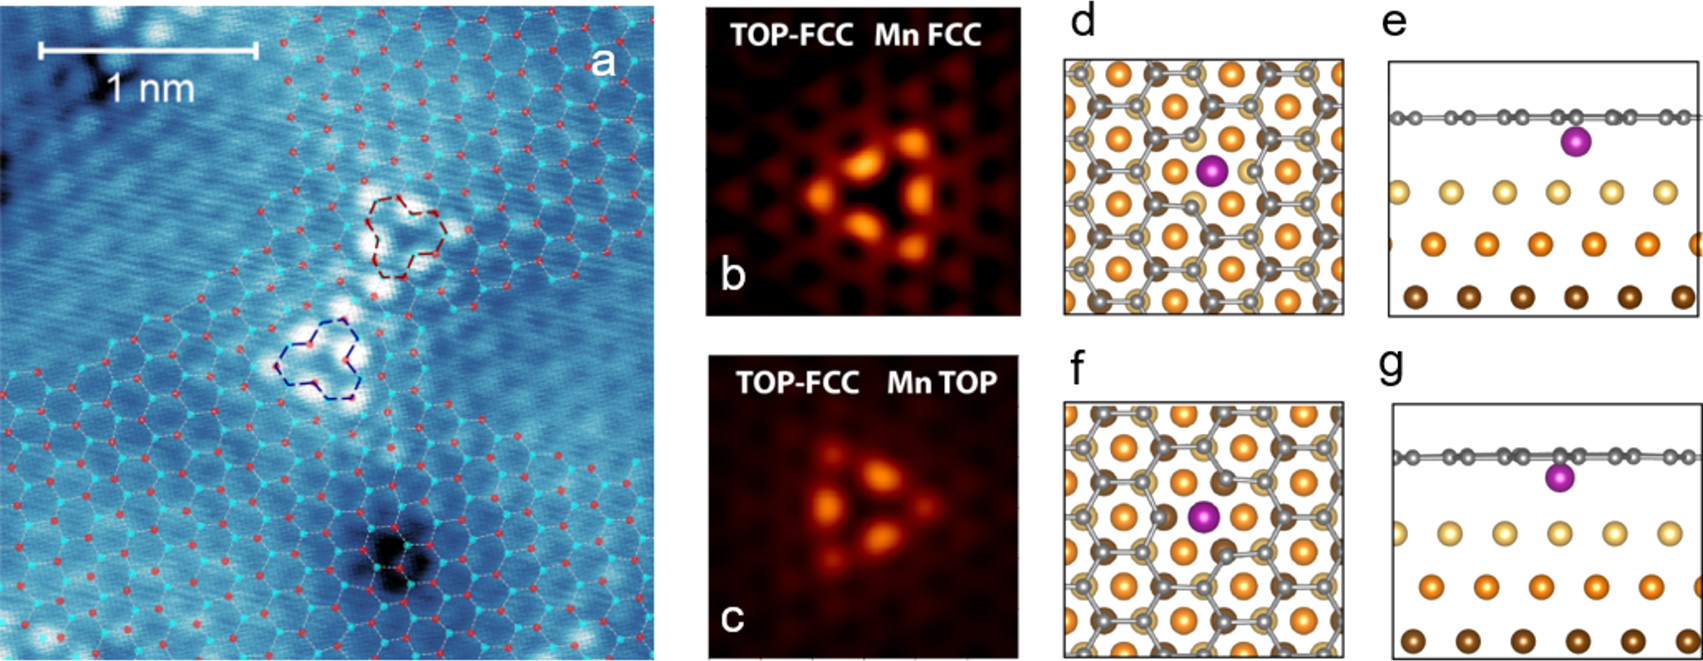
\includegraphics[width = \textwidth]{Plots/images_large_nn1c00139_0003.jpeg}
    \caption{(a) zeigt eine RTM, in welcher ersichtlich wird, dass Mn in die beiden verschiedenen Untergittern von Graphen implantiert wurde. In der
    RTM äußern sich diese mittels dreieckigen Strukturen, welche zueinander gespiegelt liegen.
    (b-c) zeigen RTM simuliert mittels Dichtefunktionaltheorie (DFT) in einer TOP-FCC Region. In (b) liegt das Mn auf einem FCC
    und in (c) auf einem TOP Gitterplatz. (d,e) zeigt das Mn auf einem FCC und (f,g) zeigt es auf einem TOP Platz in der Graphenebene und seitlich davon.
    (Abbildung entnommen  aus \cite{doi:10.1021/acsnano.1c00139})}
    \label{fig:ascnano_defect}
\end{figure}
Für die sechs verschiedenen Plätze des Mn (zwei Untergitter und drei Hochsymmetrieregionen) wurden DFT-Rechnungen für die Energien und die magnetischen Momente durchgeführt.
Dabei zeigte sich, dass diese Größen von dem lokalen Stapeln und dem Untergitter abhängen, so dass die Energie geringer ist, womit 
diese Konfiguration (z.B. Mn auf einem FCC Platz in einer TOP-FCC-Region) höhere Stabilität aufweist.
Diese Tendenz zeigte sich ebenfalls in den RTM, wobei angemerkt werden muss, dass die Datenlage dazu nicht ausreicht, um
verlässliche Ergebnisse zu haben.  
\newpage
\FloatBarrier
\section{Struktur von Graphen und der Störstelle}
\label{sec:structure}
\begin{wrapfigure}{r}{0.49\textwidth}
    \centering
    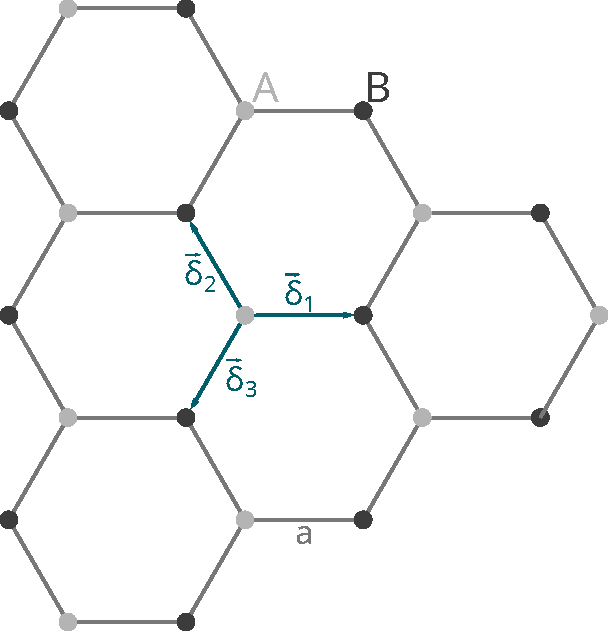
\includegraphics[width = 0.49\textwidth]{Plots/graphene_lattice.pdf}
    \caption{Das für Graphen typische Honigwabengitter. Die Kristallstruktur wird durch zwei Untergitter (A und B) und den 
    Gittervektoren $\vec{a}_1$ und $\vec{a}_2$ beschrieben, wobei
    die drei nächsten Nachbarn, die einen Abstand von $a$ (Gitterkonstante) haben, die Abstandsvektoren $\vec{\delta}_j$ besitzen.}
    \label{fig:graphene_lattice}
\end{wrapfigure}
Graphen ist ein zweidimensionales, aus einer Atomschicht bestehendes Allotrop von C, dessen
Struktur nur mit einer zweiatomigen Basis (Atom A und B) beschrieben werden kann, da sonst keine Translationsinvarianz vorherrschen würde.
Wird mit diesen inäquivalenten Atomen eine Basis gebildet, ergibt sich mit den Gittervektoren 
\begin{equation*}
        \vec{a}_1 = \frac{a}{2}\begin{pmatrix} 3 \\[4pt] \sqrt{3}  \end{pmatrix}, \quad
        \vec{a}_2 = \frac{a}{2}\begin{pmatrix} 3 \\[4pt] -\sqrt{3} \end{pmatrix}       
\end{equation*}    
ein zweidimensionales, hexagonales Gitter, welches das für Graphen typische Honigwabengitter besitzt,
wie in Abbildung \ref{fig:graphene_lattice} zu sehen ist.
Die Abstandsvektoren $\vec{\delta}_j(\varphi_j)$ der drei benachbarten B-Atome eines A-Atoms können mit Hilfe eines 
diskreten Drehwinkels $\varphi_j \in \{ 0,  \sfrac{2\pi}{3}, \, \sfrac{4\pi}{3} \} $ angegeben werden (Abb. \ref{fig:graphene_lattice}), so dass sich mit $a$ als Gitterabstand
$\vec{\delta}_j(\varphi_j) = a \, ( \sin (\varphi_j), \cos (\varphi_j) )$
ergibt.
Das Koordinatensystem kann so gelegt werden, so dass $\vec{\delta}_1$ auf der x-Achse liegt, womit sich die Abstandsvektoren mittels
\begin{equation*}
    \vec{\delta}_1 = a \begin{pmatrix} 1            \\[4pt] 0                   \end{pmatrix}, \quad
    \vec{\delta}_2 = a \begin{pmatrix} -\frac{1}{2} \\[4pt] \frac{\sqrt{3}}{2}  \end{pmatrix}, \quad 
    \vec{\delta}_3 = a \begin{pmatrix} -\frac{1}{2} \\[4pt] -\frac{\sqrt{3}}{2} \end{pmatrix}
\end{equation*}
darstellen lassen.
Wird nun aus dem Untergitter A entfernt und dort Mn eingesetzt (Abb. \ref{fig:mangan_impurity_inplane}), 
ändern sich die Abstandsvektoren, wobei es keinen Einfluss hat, auf welchem Untergitter das Mn implantiert wird.
Dies liegt, wie im vorigen Abschnitt \ref{sec:motivation} diskutiert, daran, dass das Manganatom zu groß ist und nicht in diese Stelle passt, so dass es aus der Ebene entweicht und 
eine $z$-Komponente besitzt.
Diese Situation ist in Abbildung sowohl in seitlicher Ansicht als auch in der Graphenebene  \ref{fig:mangan_impurity} dargestellt.
Die hinzukommende $z$-Komponente lässt sich mittels trigonometrischen Beziehungen zu $z = -\cot (\theta)$ bestimmen, womit die 
Abstandsvektoren durch 
\begin{equation*}
    \vec{d}_1 = a \begin{pmatrix} 1            \\[4pt] 0                   \\[4pt] \cot (\theta)\end{pmatrix}, \quad
    \vec{d}_2 = a \begin{pmatrix} -\frac{1}{2} \\[4pt] \frac{\sqrt{3}}{2}  \\[4pt] \cot (\theta)\end{pmatrix}, \quad 
    \vec{d}_3 = a \begin{pmatrix} -\frac{1}{2} \\[4pt] -\frac{\sqrt{3}}{2} \\[4pt] \cot (\theta)\end{pmatrix}
\end{equation*}
angegeben werden können.
Wie bereits in Abbildung \ref{fig:mangan_impurity} angedeutet, wird im Folgenden angenommen, dass das Mn mittig von den nächsten Nachbarn liegt, so dass 
sich die $x$- und $y$-Komponente der Abstandsvektoren nicht ändert.
\begin{figure}
    \begin{subfigure}{0.48\textwidth}%
    \centering%
    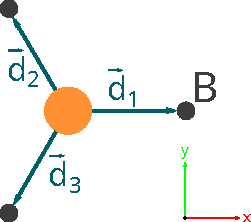
\includegraphics[height = 2.8cm]{Plots/mangan_impurity_inplane.pdf}%
    \caption{Mn-Störstelle in der Graphenebene.}%
    \label{fig:mangan_impurity_inplane}%
    \end{subfigure}%
    \hfill% Fills available space in the center -> space between figures
    \begin{subfigure}{0.48\textwidth}%
    \centering%
    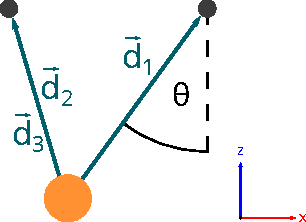
\includegraphics[height = 2.8cm]{Plots/mangan_impurity_z_component.pdf}%
    \caption{Mn-Defekt in einer seitlichen Ansicht.}%
    \label{fig:mangan_impurity_z_component}%
    \end{subfigure}%
    \caption{Darstellung des räumlichen Anordnung des Mangandefekts aus veschiedenen Ansichten.
    Aus dem Untergitter A wurde ein C entfernt und Mangan (orange) implantiert.
    Wie in Abschnitt \ref{sec:motivation} diskutiert, entweicht das Mn aus der Graphenebene.}%
    \label{fig:mangan_impurity}%
\end{figure}%
Hierbei ist es irrelevant, ob eine positive oder negative $z$-Komponente gewählt wird, da die Anordnung ohne Betrachtung des Kupfersubstrats 
spiegelsymmetrisch um die Graphenebene ist. 
Die $z$-Komponente wird negativ gewählt, damit dies konsistent mit dem Experiment ist.
Um die Bandstruktur beschreiben zu können, wird das reziproke Gitter, 
dessen Form ein um $\ang{90;;}$ gedrehtes Hexagon ist, benötigt \cite{honey}.
Dazu ist in Abbildung \ref{fig:first-brillouine-zone} die erste Brillouin-Zone mit den 
reziproken Gittervektoren (Berechung im Anhang \ref{sec:rez_lattivectors_calc})
\begin{equation*}
    \vec{b}_1 = \frac{2\pi}{3a} \begin{pmatrix}  1\\[4pt]   \sqrt{3}  \end{pmatrix}, \quad
    \vec{b}_2 = \frac{2\pi}{3a} \begin{pmatrix}  1\\[4pt] - \sqrt{3} \end{pmatrix}       
\end{equation*}    
aufgezeigt.
\begin{wrapfigure}{l}{0.4\textwidth}
    \centering
    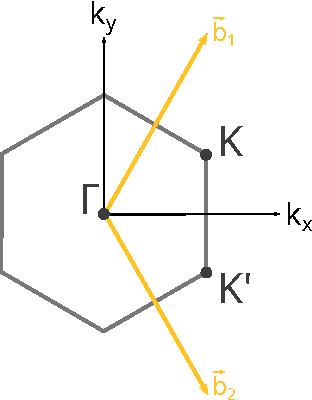
\includegraphics[width = 0.3\textwidth]{Plots/graphene_first_brillouine_zone.pdf}
    \caption{Erste Brillouin-Zone von Graphen.
    Eingezeichnet sind die reziproken Gittervektoren $\vec{b}_1$ und $\vec{b}_2$.
    Der $\symup{\Gamma}$-Punkt (Mitte der ersten Brillouine-Zone) und die beiden inäquivalenten
    Eckpunkte K und K$'$.}
    \label{fig:first-brillouine-zone}
\end{wrapfigure}
Besonders die Eckpunkte, $\vec{K} = \sfrac{2\pi}{3\sqrt{3}a} \, (\sqrt{3},1)$ 
und $\vec{K}' = \sfrac{2\pi}{3\sqrt{3}a} \, (\sqrt{3},-1)$, sind von hoher Relevanz, wie sich im folgenden Abschnitt herrausstellt.
In dieser Modellierung wird davon ausgegangen, dass Graphen komplett eben ist. 
In der Realität ist dem nicht so, da dem Mermin-Wagner Theorem nach langwellige Fluktuationen die reichtweitige Ordnung von zweidimensionalen Kristallen zerstören, womit
diese eine Krümmung aufweisen \cite{Fasolino2007}.
\FloatBarrier
\newpage
\section{Eigenschaften von Graphen}
\label{sec:propertiesofgraphene}
Der größte Teil der Bindungen von Graphen geht von den $sp^2$-Hybridorbitalen aus, mit welchen ein C mit drei umliegenden
Nachbarn in trigonalen und planaren Anordnung eine $\sigma$-Bindung eingeht \cite{RevModPhys.81.109}.
Das dazu senkrecht stehende $p$-Orbital führt zu einer weiteren Bindung, der $\pi$-Bindung, so dass ein C
mit einem der drei nächsten Nachbarn eine Doppelbindung eingeht.
Dabei sorgt das $\sigma$-Band für die Robustheit der Gitterstruktur \cite{RevModPhys.81.109}.
Aufgrund des Pauli-Prinzips haben diese Bänder eine volle Schale, welche somit ein sehr tiefes Valenzband
formen \cite{RevModPhys.81.109}.
Da jedes $p$-Orbital, welches senkrecht auf der Graphenebene steht, ein Elektron
besitzt, ist das $\pi$-Band halb gefüllt, womit sich die Elektronen frei bewegen können \cite{RevModPhys.81.109}\cite{graphene_properties}.
Dieses $\pi$-Band trägt auch mit sehr großem Anteil zu der Leitfähigkeit von Graphen bei \cite{graphene_properties}.
Die Bandstruktur kann mittels eines Tight Binding Modells ermittelt werden, woraus unter der Annahme eines nächsten-Nachbarn-Hüpfens
die Dispersionsrelation 
\begin{equation*}
    \epsilon_{\vec{k}} \propto \pm \sqrt{3+2 \cos \left ( \sqrt{3}ak_y \right )+2\cos \left ( \frac{3}{2}ak_x+\frac{\sqrt{3}}{2}ak_y \right ) + 2\cos \left ( \frac{3}{2}ak_x-\frac{\sqrt{3}}{2}ak_y \right ) }
\end{equation*}
folgt (die Rechung dazu befindet sich im Anhang \ref{sec:calc_dispersion}).
Das negative bzw. positive Vorzeichen gehört zu dem Valenz- ($\pi$) bzw. Leitungsband ($\pi^*$) \cite{RevModPhys.81.109}.
Das Valenz- und Leitungsband berühren sich in zwei inäquivalenten Punkten der ersten Brillouin-Zone K und $\text{K}'$, welche 
auch Dirac-Punkte genannt werden \cite{10.1093/nsr/nwu080}.
Wird die Dispersionsrelation um diese beiden Punkte entwickelt, nimmt die Dispersionsrelationrelation eine lineare Form an, welche mit 
\begin{equation}
    \epsilon_{\vec{k}} \propto \pm | \vec{k} | 
\end{equation}
in der Nähe der beiden Punkte die Form eines Kegels (sog. \textit{Dirac cone}) besitzt \cite{10.1093/nsr/nwu080}\cite{Avouris2007}.
Jedoch verschwindet die Zustandsdichte in diesen Punkten, wodurch Graphen als ein bandlückenloser Halbleiter mit einer verschwindenen 
Zustandsdichte am Fermi-Niveau gesehen werden kann \cite{10.1093/nsr/nwu080}. 
Aufgrund dieser linearen Dispersion können die Elektronen durch die masselose Dirac-Gleichung beschrieben werden, wobei sich 
die Elektronen (in dem Fall sog. Dirac-Elektronen) mit der Fermigeschwindigkeit $v_\text{F}$ statt der Lichtgeschwindigkeit $c$ fortbewegen,
dessen Verhältnis $\sfrac{v_\text{F}}{c} \approx \sfrac{1}{300}$ ist \cite{Avouris2007}.
Dies führt zu einer sehr hohen Ladungsträgerbeweglichkeit \cite{https://doi.org/10.1002/adma.201201482}.
Graphen ist ebenfalls aufgrund seiner makroskopischen Eigenschaften von großem Interesse und ein aktuelles Forschungsthema.
Einerseits ist die  Dichte mit $\qty{0.77}{\milli\gram\per\metre\squared}$ extrem gering, obwohl 
Graphen eine hundertfache Stärke von Stahl bei der selben Dicke aufweist \cite{graphene_properties}. 
Anderseits ist Graphen das bisher bekannte, am besten leitende Material bei Raumtemperetur mit einer Leitfähigkeit von 
$\qty{e6}{\siemens\per\metre}$ \cite{graphene_properties}.
\chapter{Struktur der Arbeit}

Eine mögliche Struktur der Arbeit sieht wie folgt aus:

\begin{enumerate}
    \item \textbf{Einleitung}\\
        In der \emph{kurzen} Einleitung wird die Motivation für die Arbeit
        dargestellt und ein Einblick in die kommenden Kapitel gegeben.
    \item \textbf{Theoretische Grundlagen}\\
        Alles was an theoretischen Grundlagen benötigt wird, sollte auch eher kurz gehalten werden.
        Statt Grundlagenwissen zu präsentieren, eher auf die entsprechenden Lehrbücher verweisen.
        Etwa: Tiefer gehende Informationen zur klassischen Mechanik entnehmen Sie bitte \cite{kuypers}.
    \item \textbf{Ergebnisse} \\
        Der eigentliche Teil der Arbeit, das was getan wurde.
    \item \textbf{Zusammenfassung und Ausblick} \\
        Zusammenfassung der Ergebnisse, Optimierungsmöglichkeiten, mögliche weitergehende Untersuchungen.
\end{enumerate}

Die Gliederung sollte auf der einen Seite nicht zu fein sein, auf der anderen Seite
sollten sich klar unterscheidende Abschnitte auch kenntlich gemacht werden.

In der hier verwendeten \KOMAScript-Klasse \texttt{scrbook} ist die oberste Gliederungsebene,
die in der Bachelorarbeit verwendet werden sollte, das \texttt{\textbackslash chapter}.

Ein Kapitel sollte erst dann in tiefere Gliederungsebenen unterteilt werden, wenn es auch wirklich etwas zu unterteilen gibt. Es sollte keine Kapitel mit nur einem Unterkapitel (\texttt{\textbackslash section}) geben.

In dieser Vorlage ist die Tiefe des Inhaltsverzeichnisses auf \texttt{chapter} und \texttt{section} beschränkt. Möchten Sie diese Beschränkung aufheben, entfernen Sie den Befehl
\begin{verbatim}
            \setcounter{tocdepth}{1}
\end{verbatim}
aus der Präambel oder ändern Sie den Zahlenwert entsprechend. Das Inhaltsverzeichnis sollte für eine Bachelorarbeit auf eine Seite passen.

\chapter{Wichtige Hinweise zum Dokument}\label{make}

Diese Vorlage ist auf die Kompilierung mit \texttt{lualatex} ausgelegt. 
Als Dokumentenklasse  wird die \KOMAScript\-Klasse \texttt{scrbook} verwendet.
Falls Sie Änderungen am Layout vornehmen möchten, lesen Sie die \KOMAScript-Dokumentation: \cite{koma}.

Eine umfangreiche Einführung in die moderne Verwendung von \LaTeX{} gibt es hier: \cite{toolbox}, lesenswert ist außerdem das \LaTeX-Tabu: \cite{l2tabu}

Um dieses Dokument vollständig zu erstellen sind maximal vier Programmläufe nötig:
\begin{enumerate}[nosep]
    \item \texttt{lualatex BachelorArbeit.tex}
    \item \texttt{biber BachelorArbeit.bcf}
    \item \texttt{lualatex BachelorArbeit.tex}
    \item \texttt{lualatex BachelorArbeit.tex}
\end{enumerate}

Beim ersten Lauf des \LaTeX-Compilers werden die Kapitel, Links und zitierten Bibliographieeinträge in Hilfsdateien geschrieben.

Dann ist ein Lauf des Programms \texttt{biber} nötig, welches die benötigten Einträge aus der Hilfsdatei einliest, die Einträge aus der \texttt{.bib} Datei einliest, sortiert und formatiert und in eine weitere Hilfsdatei schreibt.

Beim nächsten \LaTeX-Lauf werden dann diese Hilfsdateien eingelesen und Literatur- und Inhaltsverzeichnis erstellt.

Manchmal ist ein vierter Lauf nötig, falls sich durch das einfügen des Literaturverzeichnisses Seitenzahlen verändert haben.

Das Tool \texttt{latexmk} übernimmt dies mit nur einem Programmaufruf und
führ nur so viele Aufrufe durch, wie nötig sind.

\texttt{latexmk --lualatex BachelorArbeit.tex}

Eine gute Option ist es, den \LaTeX{} Output in einem anderen 
Ordner zu erzeugen, dies ist mit der \texttt{--output-directory} Option möglich:

\texttt{latexmk --output-directory=build --lualatex BachelorArbeit.tex}


\section{Erstellen des Ausgabedokuments mit Make}

Für diese Vorlage wird ein Makefile zur Verfügung gestellt, welches automatisch alle Schritte ausführt, die für das fertige Dokument nötig sind.
Die Ausgabe erfolgt dabei in den Unterordner \texttt{build/}.
Make prüft, ob die Quelldateien verändert wurden, falls nicht, werden auch keine Befehle ausgeführt.

Falls Sie das Makefile benutzen möchten, sollten Sie alle Abhängigkeiten eintragen (Eigene Dateien für Kapitel, Plots, etc.).


Download und weitere Informationen zu Make gibt es unter \cite{make}. Die Befehle sind für die Bash ausgelegt.
Wenn Sie sie unter Windows nutzen wollen, benötigen Sie einen Bash-Emulator, wie Git Bash, Download unter \cite{gitbash} möglich.
Wenn Sie Make installiert haben, rufen Sie einfach in der Konsole im Verzeichnis der Arbeit den Befehl \texttt{make}.

\section{Erstellen des Ausgabedokuments mit Texmaker}
\subsection{Einrichten der nötigen Befehle}
Ein beliebter Editor für alle Betriebssysteme ist Texmaker, Download unter \cite{texmaker}.
Damit Texmaker das Dokument korrekt kompiliert, fügen sie einen benutzerdefinierten Befehl hinzu:
\begin{enumerate}[nosep]
    \item Klicken sie oben in der Menüleiste auf \emph{Benutzer/in}
    \item Klick auf \emph{Eigene Befehle}
    \item Klich auf \emph{Eigene Befehle editieren}, dort können Sie bis zu 5 eigene Befehle definieren
    \item Geben Sie dem Befehl unter \emph{Menüeintrag} einen Namen und tragen sie folgende Befehle in das Befehlsfeld ein: \\
      \small\verb+latexmk --lualatex --interaction=batchmode --halt-on-error %.tex |+
    \item Bestätigen Sie mit \emph{OK}
\end{enumerate}

\begin{figure}
    \centering
    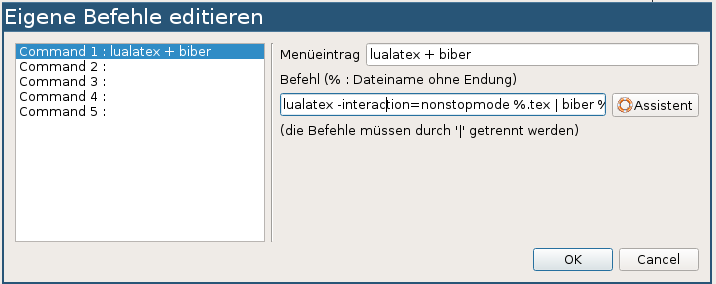
\includegraphics[width=12cm]{Plots/texmaker.png}
    \caption{Screenshot zur Erstellung des Kompilier-Befehls in Texmaker}
    \label{fig:texmaker}
\end{figure}


In Abbildung \ref{fig:texmaker} ist ein Screenshot des Befehlsmenü gezeigt. Ihren Befehl können Sie nun im Drop-Down-Menü zum 
Kompilieren des Dokuments auswählen und mit einem Klick auf den Pfeil starten.

\subsection{Aufräumen}

Nach einem \LaTeX-Fehler ist es oft notwendig, die erstellten Hilfsdateien zu löschen.
Klicken Sie hierzu auf \emph{Werkzeuge}→\emph{Aufräumen}.


\chapter{\LaTeX-Grundlagen}

Bitte beachten Sie beim Schreiben der Arbeit folgende Konventionen bzw. Grundlagen:

\begin{itemize}
    \item \textbf{Abschnitte und Zeilenumbrüche} \\
        Es sollten im Fließtext keine Zeilenumbrüche mit \textbackslash\textbackslash \ erzwungen werden.
        Schreiben Sie höchsten einen Satz in eine Code-Zeile.
        Absätze werden im Code mit einer Leerzeile markiert und dann entsprechend der Einstellung von \texttt{parskip} in der Dokumentenklasse gesetzt.
    \item \textbf{Kursiv/Aufrecht} \\
        \begin{itemize}
            \item Variablen und physikalische Größen werden kursiv gesetzt. 
            \item Einheiten werden immer aufrecht und mit einem halben Leerzeichen Abstand zur Zahl gesetzt. Nutzen Sie \texttt{siunitx}!
            \item Mathematische Konstanten und Funktionen werden ebenfalls aufrecht gesetzt. Zum Beispiel die Eulersche Zahl e, das imaginäre i und das infinitesimale d.
                Im Mathematikmodus können Sie dies mit dem Befehl \verb_\mathrm{}_ erreichen. Für die Funktionen stellt \LaTeX \ Befehle bereit, z.B. \verb+\arccos+.
            \item Integrand und ein $\mathrm{d}x$ sollten ebenfalls durch ein kleines Leerzeichen (\verb+\,+) getrennt werden.
        \end{itemize}
        


\end{itemize}

\section{Zahlen und Einheiten}

Jede Zahl, jede Einheit und jede Zahl mit Einheit sollte mit Hilfe der in dem Paket \texttt{siunitx} zur Verfügung gestellten Befehle gesetzt werden.
Grundsätzlich gilt: Einheiten werden aufrecht gesetzt und haben ein kleines Leerzeichen (\verb+\,+) Abstand zu ihrer Zahl. 
Werden Fließkommazahlen ohne \texttt{siunitx} gesetzt, entsteht ein hässlicher Leerraum zwischen Komma und erster Nachkommastelle, da \LaTeX \ das Komma nicht als Dezimaltrennzeichen, sondern als Satzzeichen interpretiert.

Das Paket wurde mit deutschen Spracheinstellungen (also mit Komma als Dezimaltrennzeichen und $\cdot$ zwischen Zahl und Zehnerpotenz) geladen, sowie mit den Einstellungen, dass die Standardabweichung stets durch $\pm$ abgetrennt wird und Einheiten falls nötig als Brüche ausgegeben werden.

\begin{table}
    \centering
    \caption{Beispiele für siunitx}
    \label{tab:si}
    \begin{tabular}{l r}
        \toprule
        Befehl     &   Ergebnis \\
        \midrule
        \verb+\num{1.2345}+ & \num{1.2345} \\
        \verb+\num{1.2e3}+ & \num{1.2e3} \\
        \verb_\num{1.2 +- 0.2}_ & \num{1.2+-0.2} \\
        \verb+\num{10000}+ & \num{10000} \\
        \verb+\si{\meter\per\second}+ & \si{\meter\per\second} \\
        \verb+\SI{1.2(1)}{\micro\ampere}+ & \SI{1.2(1)}{\micro\ampere} \\
        \verb+\SI{1.2\pm0.1e3}{\kilo\gram\per\cubic\meter}+ & \SI{1.2\pm0.1e3}{\kilo\gram\per\cubic\meter} \\
        \bottomrule 
    \end{tabular}
\end{table}

Das Paket stellt unter anderem die drei wichtigen Befehle
\begin{itemize}
    \item \texttt{\textbackslash num\{Zahl\}},
    \item \texttt{\textbackslash si\{Einheit\}} und
    \item \texttt{\textbackslash SI\{Zahl\}\{Einheit\}}
\end{itemize}
zur Verfügung.
Diese Befehle sollten stets genutzt werden, wenn Zahlen angegeben werden. 
Sie funktionieren sowohl im Text- als auch im Mathematikmodus.
In Tabelle \ref{tab:si} sind einige Beispiele aufgetragen. Bitte lesen Sie die Dokumentation \cite{siunitx}.

\section{Das Literaturverzeichnis}

Das Literaturverzeichnis wird mit Hilfe von BibLaTeX und biber erstellt.
Tragen Sie alle ihre Quellen in die Datei \texttt{references.bib} ein, Sie enthält bereits
einige Beispiele. Für weitere Informationen lesen Sie bitte die Dokumentation \cite{biblatex}.

Im Text können Sie mit \verb_\cite{kürzel}_ zitieren. Seitenzahlen geben Sie in eckigen Klammern an:
\verb_\cite[10]{kürzel}_. 

Das Literaturverzeichnis ist so eingestellt, dass es Ihre Quellen in alphabetischer Reihenfolge nach Autoren nummeriert.
Möchten Sie das Literaturverzeichnis nach der Reihenfolge des Auftauchens im Text sortieren, fügen sie die Paktetoption \texttt{sorting=none} beim Laden
des BibLaTeX-Pakets hinzu.

Den Zitier- und Bibliographie-Stil geben sie mit der Option \texttt{style=Stil} an. Die beiden gebräuchlisten Stile sind \texttt{numeric} und \texttt{alphabetic}. 
Bei \texttt{numeric} werden die Quellen durchnummeriert, bei \texttt{alphabetic} wird ein Buchstabenkürzel aus Autor(en)-Name(n) und Jahr verwendet.
Für weitere Stile konsultieren Sie bitte die Dokumentation: \cite{biblatex}.

Ein Beispiel für das Zitieren eines Buches lautet so \cite{handbook_adhesives},
wissenschaftliche Artikel hingegen werden so \cite{einstein} zitiert.

Damit das Literaturverzeichnis erstellt wird, ist ein Aufruf von \texttt{biber} nach einem ersten kompilieren mit \texttt{lualatex} nötig.
Danach muss das Dokument erneut mit \texttt{lualatex} kompiliert werden. 

Zum korrekten Kompilieren des Dokuments siehe Kapitel \ref{make}.

\chapter{Abbildungen und Tabellen}

\section{Abbildungen}

Achten Sie bei ihren Plots auf ausreichend große Achsenbschriftungen, ausreichende Schriftdicken und gut unterscheidbare Farben.
Im Idealfall haben Sie im Plot und der Arbeit die gleiche Schriftgröße und Schriftart.
Dies lässt sich durch Erstellen des Plots in der korrekten Größe und Einbinden mit dem optionalen Argument \texttt{scale=1} erreichen. Ein Beispiel sehen Sie in Abbildung \ref{fig:bsp}.

Nutzen Sie wenn möglich Vektorgrafiken (pdf) und nur in Ausnahmen Rastergrafiken wie .png oder .jpg.
Setzen Sie Punkte hinter Abbildungsunterschriften.

\begin{figure}
    \centering
    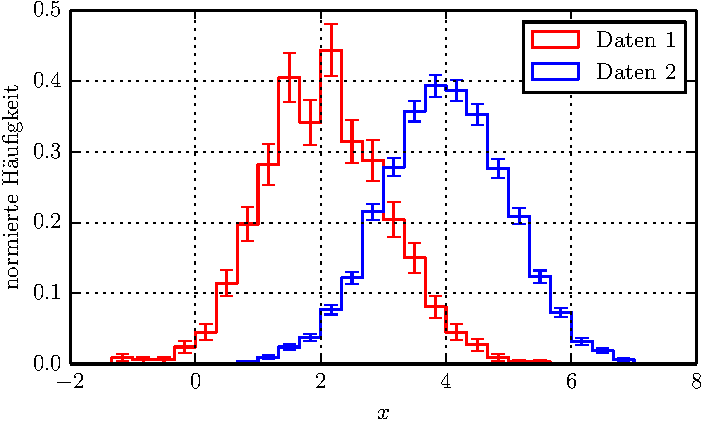
\includegraphics[scale=1]{./Plots/Histogramm.pdf}
    \caption{Ein Histogramm mit Fehlerbalken für zwei Datensätze, Schriftgröße und -art entsprechen der des Dokuments.}
    \label{fig:bsp}
\end{figure}

\section{Tabellen}

Tabellen sollten so einfach wie möglich aufgebaut sein, verzichten Sie auf zu viele Linien. In fast allen Fällen reichen drei horizontale Linien aus, jeweils über und unter der Tabelle und zwischen den Spaltenüberschriften und der eigentlichen Tabelle.

Das Paket \texttt{booktabs} stellt hierfür \verb_\toprule_, \verb_\midrule_ und 
\verb_\bottomrule_ zur Verfügung.
Das Paket \texttt{siunitx} stellt eine extrem mächtige neue Spalteneinstellung bereit: \texttt{S}, mit ihr können Zahlen und Einheiten sehr sauber und gut ausgerichtet gesetzt werden.

Diese Vorlage geht von Tabellenüberschriften aus, möchten Sie dagegen Tabellenunterschriften entfernen Sie das entsprechende optionale Argument für die Dokumentenklasse in der Präambel.

Ein Beispiel ist Tabelle~\ref{tab:bsp}.
\begin{table}
    \centering
    \caption{Beispieltabelle mit willkürlichen Werten, für die Zahlenwerte wurde die S-Option aus \texttt{siunitx} verwendet.}
    \label{tab:bsp}
    \begin{tabular}{S[table-format=4.2] S[table-format=3.2]}
        \toprule
        {$p \mathrel{/} \si{\pascal}$}  & {$T \mathrel{/} \si{\kelvin}$} \\
        \midrule
        1024,23 & 273,15 \\
        1025,31 & 274,5 \\
        1026,27 & 276,2 \\
        \bottomrule
    \end{tabular}
\end{table}

\chapter{Berechnung}
\label{chap:berechnung}
\section{Tight-Binding-Hamiltonian}
\label{sec:hamiltonian}
Der Hamiltonian in Ortsdarstellung ist 
\begin{equation}
    H = \sum_m \epsilon_m d_m^\dagger d_m - t \sum_{i,j} \left ( c_i^\dagger c_j + c_j^\dagger c_i \right )
    + \sum_{m,j} \left ( V_{mj} d_m^\dagger c_j + V^*_{mj} c_j^\dagger d_m  \right)
\end{equation}
\cite{anders-fkt}
\appendix
% Hier beginnt der Anhang, nummeriert in lateinischen Buchstaben
\chapter{Anhang}
\section{Berechnung der reziproken Gittervektoren}
\label{sec:rez_lattivectors_calc}
Ausgehend von den Gittervektoren des Realraums 
\begin{equation*}
    \vec{a}_1 = \frac{a}{2}\begin{pmatrix} 3 \\[4pt] \sqrt{3}  \end{pmatrix}, \quad
    \vec{a}_2 = \frac{a}{2}\begin{pmatrix} 3 \\[4pt] -\sqrt{3} \end{pmatrix}       
\end{equation*}   
können die reziproken Gittervektoren mittels $\underline{\underline{B}} = 2\pi \left ( \underline{\underline{A}}^\text{T} \right )^{-1} $ \cite{suter}.
In der Matrix $\underline{\underline{A}}$ sind die Gittervektoren in den Spalten aufgetragen.
Somit folgt 
\begin{equation*}
    \underline{\underline{B}} = 2 \pi a
    \begin{pmatrix}
        \frac{3}{2} & \frac{\sqrt{3}}{2}  \\[0.35em]
        \frac{3}{2} & -\frac{\sqrt{3}}{2}
    \end{pmatrix}^{\! -1} \; .
\end{equation*}
Zur Berechnung der Inversen kann die Cramersche Regel für $2\times 2$ Matritzen angewendet werden, womit sich die gesuchte Matrix zu
\begin{equation*}
    \underline{\underline{B}} = - \frac{4\pi}{a3\sqrt{3}}
    \begin{pmatrix}
        -\frac{\sqrt{3}}{2} & -\frac{\sqrt{3}}{2}  \\[0.35em]
        -\frac{3}{2} & \frac{3}{2}
    \end{pmatrix}
\end{equation*}
ergibt \cite{Cramer}.
Die Spalten sind die reziproken Gittervektoren mit 
\begin{equation*}
    \vec{b}_1 = \frac{2\pi}{3a}\begin{pmatrix} 1        \\[4pt]     \sqrt{3}  \end{pmatrix}, \quad
    \vec{b}_2 = \frac{2\pi}{3a}\begin{pmatrix} 1        \\[4pt] -   \sqrt{3} \end{pmatrix}   \; .  
\end{equation*}
\section{Berechnung der Dispersionsrelation von Graphen}
\label{sec:calc_dispersion}
Der Tight Binding Hamiltonian für Graphen lautet
\begin{equation*}
   H= - t \sum_{i=1}^N \sum_{j=1}^N\left ( c_i^\dagger c_j + c_j^\dagger c_i \right ) \; .
\end{equation*}
Dazu wird der Ansatz einer Fouriertransformation 
\begin{equation*}
    c_i = \frac{1}{\sqrt{N}} \sum_{\vec{k}}^{1. \, \text{BZ}} \symup{e}^{\symup{i}\vec{k}\vec{l}} c_{\text{A}, \vec{k}} \; , 
    \quad c_n = \frac{1}{\sqrt{N}} \sum_{\vec{k}}^{1. \, \text{BZ}} \symup{e}^{\symup{i}\vec{k}(\vec{l}+\vec{\delta}_j)} c_{\text{B}, \vec{k}}
\end{equation*}
gemacht. 
Dieser Wird in den Hamiltonian eingesetzt, womit 
\begin{align*}
    H &= -\frac{t}{N} \sum_{j\vec{l}} \sum_{\vec{k}\vec{k}'} ( \symup{e}^{-\symup{i}\vec{k}\vec{l}}c^\dagger_{A,\vec{k}} 
    \symup{e}^{\symup{i}\vec{k}'(\vec{l}+\vec{\delta}_j)}c_{B,\vec{k}'} + \symup{e}^{-\symup{i}\vec{k}'(\vec{l}+\vec{\delta}_j)} c^\dagger_{B,\vec{k}'} 
    \symup{e}^{\symup{i}\vec{k}\vec{l}}c_{A,\vec{k}}) \\
    &= -\frac{t}{N} \sum_{j\vec{l}} \sum_{\vec{k}\vec{k}'} ( \symup{e}^{-\symup{i}(\vec{k}- \vec{k}')\vec{l}}\symup{e}^{\symup{i}\vec{k}\vec{\delta}_j}c^\dagger_{A,\vec{k}} c_{B,\vec{k}'} + 
    \symup{e}^{\symup{i}(\vec{k}- \vec{k}')\vec{l}} \symup{e}^{-\symup{i}\vec{k}\vec{\delta}_j} c^\dagger_{B,\vec{k}'}c_{A,\vec{k}}) \\
    &= -t \sum_{j\vec{k}} ( \symup{e}^{\symup{i}\vec{k}\vec{\delta}_j}c^\dagger_{A,\vec{k}} c_{B,\vec{k}} + 
    \symup{e}^{-\symup{i}\vec{k}\vec{\delta_j}} c^\dagger_{B,\vec{k}}c_{A,\vec{k}})
\end{align*}
folgt.
In dem letzten Schritt wurde $\sum_{\vec{l}}^N \symup{e}^{-\symup{i}(\vec{k}- \vec{k}')\vec{l}} 
= \sum_{\vec{l}}^N \symup{e}^{\symup{i}(\vec{k}- \vec{k}')\vec{l}} = N\delta_{\vec{k}, \vec{k}'}$ ausgenutzt, so dass die Summe über $\vec{k}'$ verschwindet.
Der Hamiltonian kann in die Form 
\begin{equation*}
    H = \sum_{\vec{k}} \begin{pmatrix}
        c_{\text{A},\vec{k}}^{\dagger} & c_{\text{B},\vec{k}}^{\dagger}
    \end{pmatrix}
    \begin{pmatrix}
        0 & -t\sum_{j} \symup{e}^{\symup{i}\vec{k}\vec{\delta}_j}     \\
        -t\sum_{j} \symup{e}^{-\symup{i}\vec{k}\vec{\delta}_j} & 0     
    \end{pmatrix}
    \begin{pmatrix}
        c_{\text{A},\vec{k}} \\
        c_{\text{B},\vec{k}}
    \end{pmatrix}
\end{equation*}
gebracht werden.
Die Eigenwerte der auftretenden $2 \times 2$-Matrix bilden die Dispersionsrelation.
Somit kann diese Matrix gemäß
\begin{equation*}
    \begin{vmatrix}
        -\varepsilon_{\vec{k}} & -t\sum_{j} \symup{e}^{\symup{i}\vec{k}\vec{\delta}_j}     \\
        -t\sum_{j} \symup{e}^{-\symup{i}\vec{k}\vec{\delta}_j} & -\varepsilon_{\vec{k}}     
    \end{vmatrix} \stackrel{!}{=} 0 
    \iff \varepsilon_{\vec{k}}^2 - t^2 \left | \sum_{j} \symup{e}^{\symup{i}\vec{k}\vec{\delta}_j} \right |^2 = 0 
    \iff \varepsilon_{\vec{k}} = \pm t \left | \sum_{j} \symup{e}^{\symup{i}\vec{k}\vec{\delta}_j} \right |
\end{equation*}
diagonalisiert werden.
Die Summe ausgeschrieben ergibt
\begin{equation*}
    \varepsilon_{\vec{k}} = \pm t \sqrt{3+2 \cos \left ( \sqrt{3}ak_y \right )+2\cos \left ( \frac{3}{2}ak_x+\frac{\sqrt{3}}{2}ak_y \right ) + 2\cos \left ( \frac{3}{2}ak_x-\frac{\sqrt{3}}{2}ak_y \right ) } \; \; .
    \label{eqn:dispersion_graphene_calc}
\end{equation*}


\backmatter
\printbibliography

\cleardoublepage
\thispagestyle{empty}
\section*{Eidesstattliche Versicherung}
Ich versichere hiermit an Eides statt, dass ich die vorliegende Abschlussarbeit mit dem Titel \enquote{\thetitle} selbstständig und ohne unzulässige fremde Hilfe erbracht habe.
Ich habe keine anderen als die angegebenen Quellen und Hilfsmittel benutzt, sowie wörtliche und sinngemäße Zitate kenntlich gemacht. 
Die Arbeit hat in gleicher oder ähnlicher Form noch keiner Prüfungsbehörde vorgelegen.

\vspace*{1cm}\noindent
\begin{center}
  \begin{tabular}{@{}p{0.4\textwidth}@{\hspace{0.15\textwidth}}p{0.4\textwidth}@{}}
  \rule{\linewidth}{0.25pt}& \rule{\linewidth}{0.25pt}\\
  Ort, Datum & Unterschrift
  \end{tabular}
\end{center}

\subsection*{Belehrung}
Wer vorsätzlich gegen eine die Täuschung über Prüfungsleistungen betreffende Regelung einer Hochschulprüfungsordnung verstößt, handelt ordnungswidrig.
Die Ordnungswidrigkeit kann mit einer Geldbuße von bis zu \SI[round-mode=places, round-precision=2]{50000}{€} geahndet werden. 
Zuständige Verwaltungsbehörde für die Verfolgung und Ahndung von Ordnungswidrigkeiten ist der Kanzler/die Kanzlerin der Technischen Universität Dortmund. 
Im Falle eines mehrfachen oder sonstigen schwerwiegenden Täuschungsversuches kann der Prüfling zudem exmatrikuliert werden \mbox{(\S\,63 Abs. 5 Hochschulgesetz --HG--).}

Die Abgabe einer falschen Versicherung an Eides statt wird mit Freiheitsstrafe bis zu 3 Jahren oder mit Geldstrafe bestraft.

Die Technische Universität Dortmund wird ggf.\ elektronische Vergleichswerkzeuge (wie z.\,B.\ die Software \enquote{turnitin}) zur Überprüfung von Ordnungswidrigkeiten in Prüfungsverfahren nutzen. \\[\baselineskip]

\noindent Die oben stehende Belehrung habe ich zur Kenntnis genommen.\\[1cm]
\begin{center}
\begin{tabular}{@{}p{0.4\textwidth}@{\hspace{0.15\textwidth}}p{0.4\textwidth}@{}}
\rule{\linewidth}{0.25pt}& \rule{\linewidth}{0.25pt}\\
Ort, Datum & Unterschrift
\end{tabular}
\end{center}

\end{document}
